\section{Exploratory data analysis}\label{sec:2}

This section follows the six EDA activities from the course. The full analysis is in \texttt{analysis/01\_eda.ipynb}. Here we show the findings that changed how we modelled the problem, and for each one we explain what it meant for our choices.

\subsection{Domain knowledge (search domain knowledge)}\label{sec:2.1}

Three ideas from hydropower scheduling are needed to understand the data and the rest of the report. We took them from the dataset description \citep{sintef2026dataset}, SINTEF's paper on this dataset \citep{barjaktarevic2026} and literature on hydropower scheduling.

\textbf{Water value.} Water in a reservoir can be used to produce power now or saved for later. The \emph{water value} (EUR/MWh) is what the water is expected to be worth if it is saved. A plant should therefore produce when the electricity price is higher than the water value of the water it uses, and save the water otherwise. This is the core economic rule behind the scheduling decisions, and we test it directly in Section~\ref{sec:2.5}.

\textbf{Start costs.} Starting a unit costs money, mainly through wear on the equipment. A scheduler therefore avoids switching a unit on for a single hour, so decisions should come in long blocks rather than follow every change in price.

\textbf{The cascade.} The plants are connected: water released by one plant flows into the reservoir of the next (Songa $\rightarrow$ Totak $\rightarrow$ Vinje $\rightarrow$ Vinjevatn $\rightarrow$ Tokke $\rightarrow$ Bandak $\rightarrow$ Hogga). A plant's decision therefore depends on what the plants above and below it do. The most important example is Vinje and Tokke: Vinje releases into Vinjevatn, a small reservoir (9.4~Mm³) that Tokke can empty in about 20 hours, so the two plants must largely run together.

\subsection{How the data was generated (understand how the data was generated)}\label{sec:2.2}

\textbf{The labels come from an optimiser.} The on/off decisions are not measured operation but the output of SHOP. For each case, SHOP received the prices and inflows for the whole week in advance, the reservoir volumes at the start, and the water values, and computed the most profitable schedule. The labels are therefore, in principle, a deterministic function of the inputs, and the task is closer to imitating an optimiser than to forecasting. This is what led us to build our own simplified version of SHOP's problem (Section~\ref{sec:5.lp}).

\textbf{The water values follow a formula.} The water values are synthetic. Dividing each one by the mean price of the following week gives a ratio between 0 and 2 with a median of 1.00 (Figure~\ref{fig:2.1}). In other words, the water value is roughly $c \times$ next week's mean price, where $c$ says how scarce the water is: close to 2 when the reservoir is low and close to 0 when it is full. The 17 reservoir columns contain only 9 distinct series. This has two consequences. First, the water value contains the price level, so comparing the price with the water value removes the price level. Second, the value at start + 7 days is the one used to value the water left at the end of the week, and it turned out to be far more predictive than the start-day value (Section~\ref{sec:2.5}).

\begin{figure}[H]
  \centering
  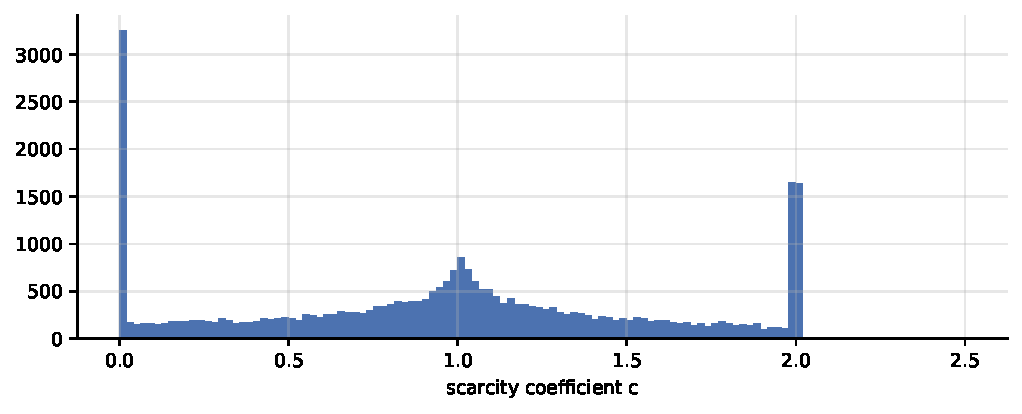
\includegraphics[width=\linewidth]{figures/fig_2_1.pdf}
  \caption{Water value divided by next week's mean price, all reservoirs and days (median 1.00, 1st percentile 0.00, 99th percentile 2.00)}
  \label{fig:2.1}
\end{figure}

\textbf{Overlapping cases are solved independently.} A new case starts every day and lasts seven days, so neighbouring cases share six days. They nevertheless disagree on about 12\% of the shared unit-hours (Figure~\ref{fig:2.2}). The disagreement is largest for Tokke and Vinje (82--85\% agreement) and smallest for the small plants (94--96\%). A possible explanation is that each case has its own start state and end-of-week valuation, and when two schedules are almost equally profitable the optimiser can pick either. Tokke and Vinje have several identical units and therefore the most near-ties. This has two consequences: it limits how well any model can do, and it means that a random split of cases would leak, because a validation case would share six days of inputs with training cases. We therefore validate by year, with a buffer between training and validation (Section~\ref{sec:3}).

\begin{figure}[H]
  \centering
  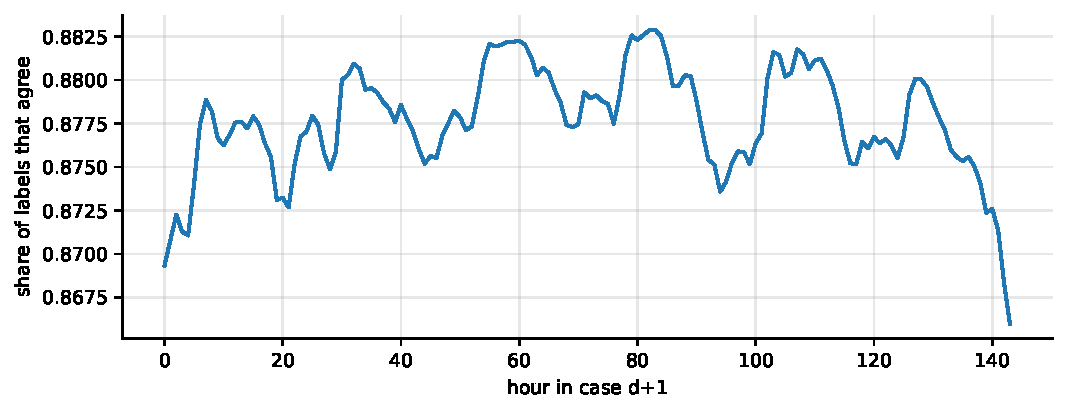
\includegraphics[width=\linewidth]{figures/fig_2_2.pdf}
  \caption{Label agreement between case d+1 and case d on the same clock hour (overall 87.8\%)}
  \label{fig:2.2}
\end{figure}

\textbf{Solver time.} The training labels come with SHOP's calculation time. The median is 52 seconds, but there is a long tail up to about 4500 seconds and a cluster near 1000 seconds that looks like a time limit. Labels from these runs may be less optimal. The calculation time is not available for the test cases, so we never used it as a feature.

\subsection{Is the data intuitive? (check if the data is intuitive)}\label{sec:2.3}

\textbf{The values are physically possible.} There are no negative inflows or water values, and the labels are only 0 or 1. The one surprise was that the volume exceeds the stated maximum in 14 of the 17 reservoirs, by up to 18\% for Bandak. This happens on few days, mostly during floods. The maximum is the highest \emph{regulated} level, so a lake can briefly rise above it. We therefore kept these values, and our LP allows them.

\textbf{The decisions make economic sense, but only when price and water value are read together} (Figure~\ref{fig:2.3}). Panel (a) shows that the share of hours on does not follow the price, but follows which of price and water value is higher. In 2020, a very wet year, prices were close to zero, yet units were on 60--80\% of the time in most months, because the water value was even lower: the reservoirs were full and the water had to be used. In 2022 prices were record high, yet units were on only 9--44\% of the time from January to September, because the water value was higher still. Panel (b) shows a typical week for one unit: the on-blocks line up with the hours where the price is above the water value. The hours where they disagree lie close to the line, where running makes little difference to the profit, or are explained by start costs. Panels (c) and (d) show the same over all cases: against price alone the share on is flat or even falling, while against price minus water value it forms a clean S-curve that crosses 50\% at zero.

\begin{figure}[H]
  \centering
  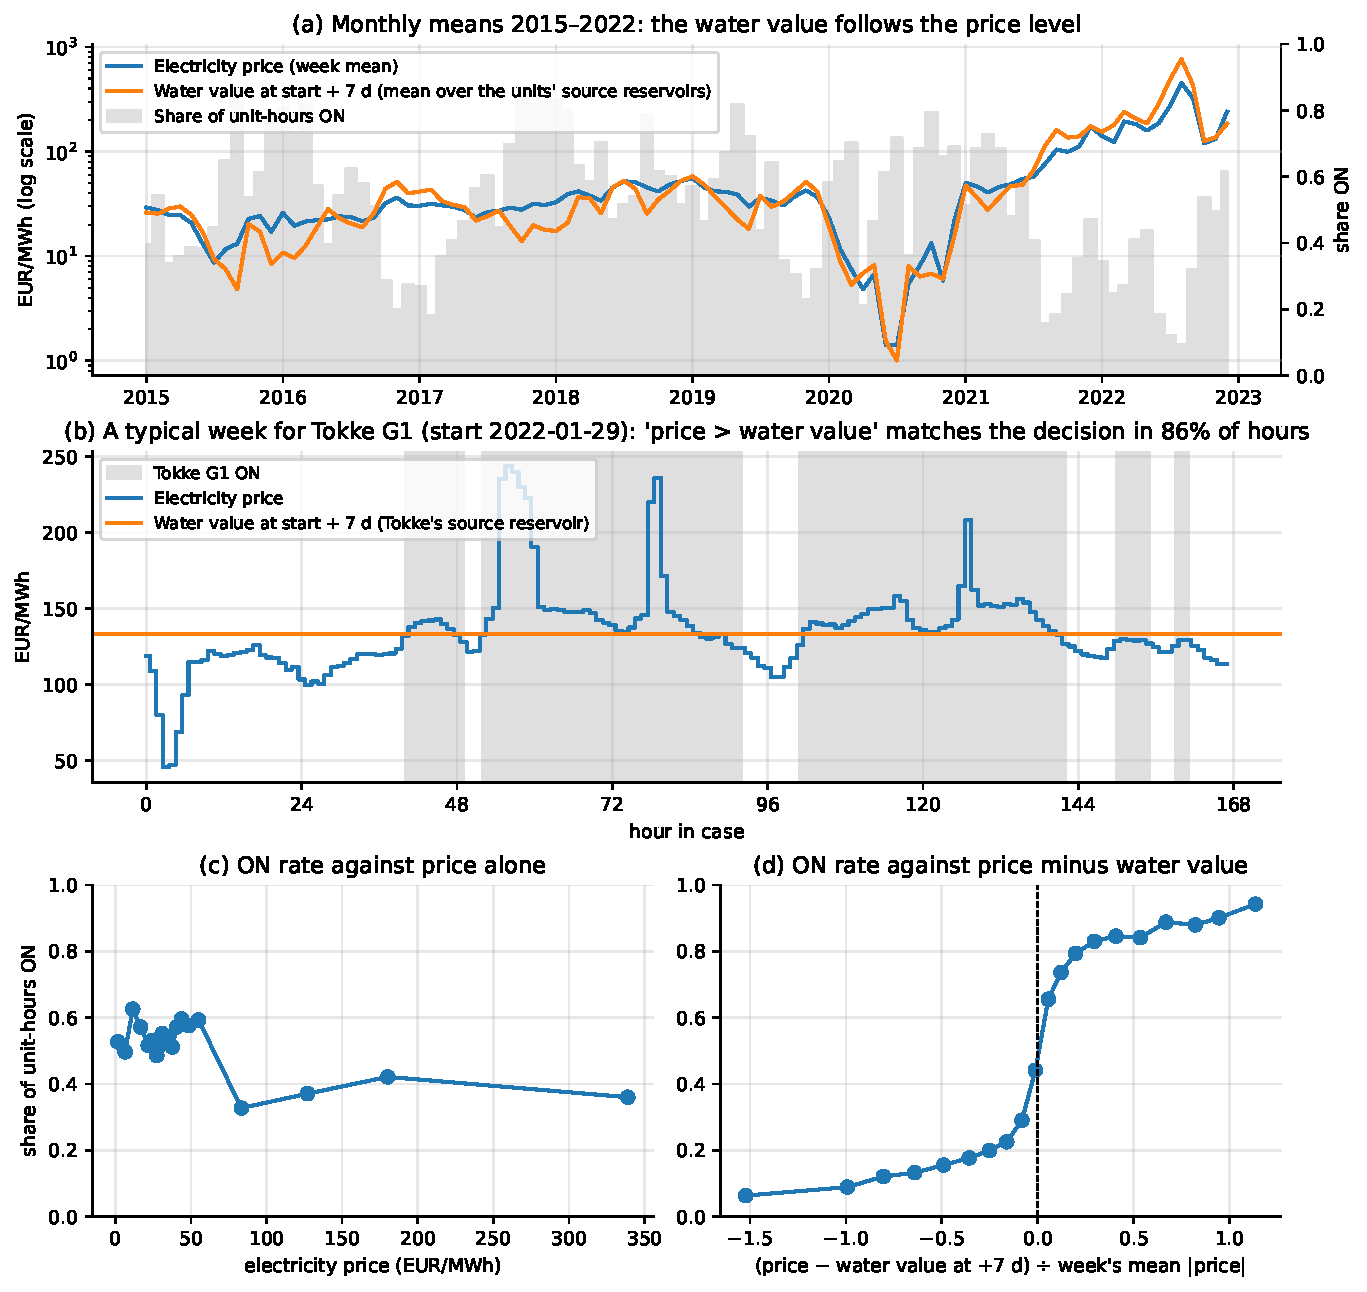
\includegraphics[width=\linewidth]{figures/fig_2_3.pdf}
  \caption{Electricity price, water value and on/off decisions}
  \label{fig:2.3}
\end{figure}

\textbf{The decisions are ``sticky''.} Only 1.2\% of the hours switch between on and off, and in 59\% of the unit-weeks a unit never switches. This matches the start costs (Section~\ref{sec:2.1}), and it means the decision in one hour depends strongly on the neighbouring hours, which a single-hour rule cannot capture.

\textbf{Identical units follow a fixed priority order.} Tokke has four and Vinje three identical units, yet their shares on differ a lot. Table~\ref{tab:2.1} shows why: a unit is almost never on while the unit before it in the order is off. Tokke G1 always starts first, then G3, G4 and G2. A model therefore has to know which unit it is predicting for, and the LP needs this order to turn a plant's ``number of units on'' into decisions per unit.

\begin{table}[H]
  \centering\small
  \caption{Priority order within the multi-unit plants}
  \label{tab:2.1}
  \adjustbox{max width=\linewidth}{\begin{tabular}{llll}
\toprule
\textbf{unit} & \textbf{higher-priority unit} & \textbf{P(unit ON while higher-priority unit OFF)} & \textbf{ON rate of unit} \\
\midrule
Vinje\_G2 & Vinje\_G1 & 0.07\% & 0.42 \\
Vinje\_G3 & Vinje\_G2 & 0.02\% & 0.26 \\
Tokke\_G3 & Tokke\_G1 & 0.05\% & 0.56 \\
Tokke\_G4 & Tokke\_G3 & 0.29\% & 0.50 \\
Tokke\_G2 & Tokke\_G4 & 1.87\% & 0.48 \\
Tokke\_G2 & Tokke\_G1 & 0.03\% & 0.48 \\
\bottomrule
\end{tabular}
}
\end{table}

\subsection{Individual features (explore individual features)}\label{sec:2.4}

\textbf{Target.} Overall, units are on 51.6\% of the time, so the classes are balanced. The share varies from 26\% (Vinje G3) to 75\% (Lio), and much more between years than between months: from 63\% in 2018 to 34\% in 2022 (Figure~\ref{fig:2.4}). Single units change even more, for example Haukeli from 87\% in 2015 to 14\% in 2022. A model can therefore not just learn that a unit is usually on; it has to learn \emph{why} from price, water value and reservoirs. This is also why we validate on whole years. Within the week, the share on follows a daily cycle with peaks in the morning and evening, but there is no trend from the first to the last hour of the case.

\begin{figure}[H]
  \centering
  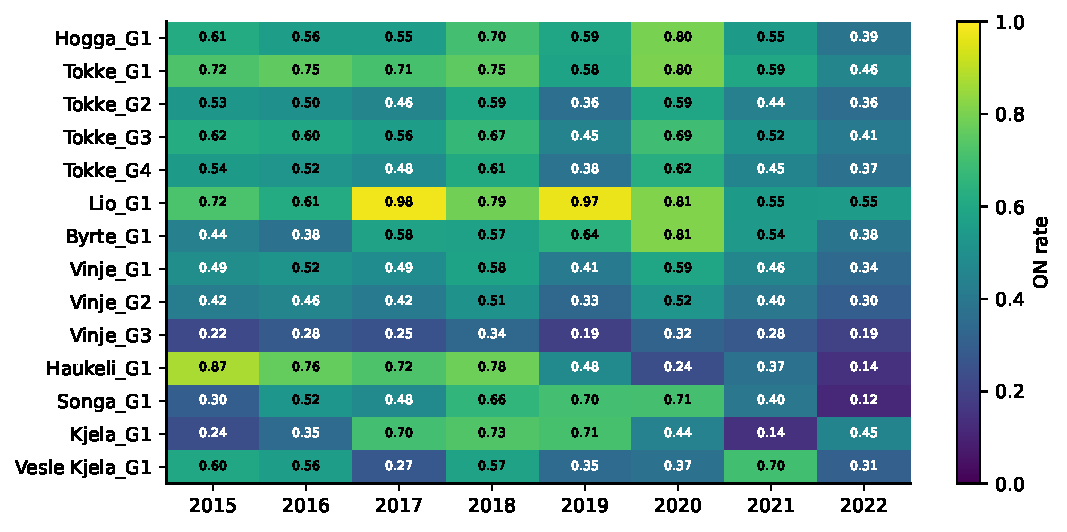
\includegraphics[width=\linewidth]{figures/fig_2_4.pdf}
  \caption{Share of hours on per unit and year}
  \label{fig:2.4}
\end{figure}

\textbf{Price.} The price has very different regimes: a yearly mean of 20--43~EUR/MWh in 2015--2019, 9 in 2020, 211 in the 2022 energy crisis, and 79 and 50 in the test years 2023 and 2024 (Figure~\ref{fig:2.5}). The test years also contain about 380 hours with negative prices, compared with about 10 in all training years. A model trained on raw prices would see test prices in a range it has rarely seen, so we use relative price features instead (Section~\ref{sec:4}).

\begin{figure}[H]
  \centering
  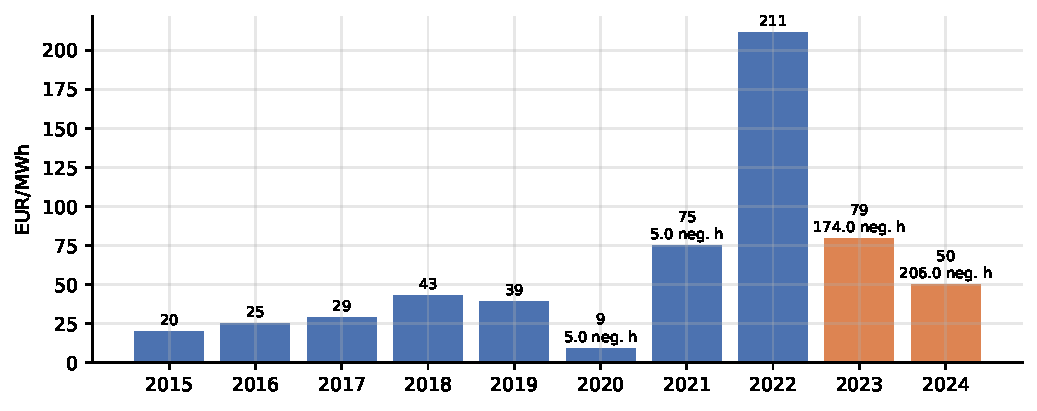
\includegraphics[width=\linewidth]{figures/fig_2_5.pdf}
  \caption{Mean day-ahead price per year (blue = training years, orange = test years)}
  \label{fig:2.5}
\end{figure}

\textbf{Inflow, volume and constraints.} Inflow is dominated by snowmelt: about 15 times higher in May--June than in January--March. The reservoirs follow the same cycle, emptiest in April (about 36\% full) and fullest in October--November (about 85\%). 2022 had the lowest fill (58\% on average), which fits with the few units on that year. The minimum-flow and minimum-volume constraints follow the same seasonal calendar every year, so on their own they carry little information beyond the time of year. They matter mainly through the LP, where they limit how water can be used.

\subsection{Pairs and groups of features (explore pairs and groups of features)}\label{sec:2.5}

\textbf{Price minus water value is the core signal.} Table~\ref{tab:2.2} ranks all unit-hours by single candidate rules and measures each with the competition metric (AUC). Price alone gives 0.454, slightly worse than guessing, because high prices (2022) come with even higher water values (Figure~\ref{fig:2.3}a). Price minus the upstream water value at start + 7 days gives 0.872. This was the most important EDA finding: the signal lies in the \emph{relationship} between two inputs, not in either one, exactly as the domain knowledge in Section~\ref{sec:2.1} suggests. It became the first baseline (Section~\ref{sec:5.rule}) and the basis of our margin features.

\begin{table}[H]
  \centering\small
  \caption{Each candidate as a single rule, ranked over all units together}
  \label{tab:2.2}
  \adjustbox{max width=\linewidth}{\begin{tabular}{ll}
\toprule
\textbf{} & \textbf{AUC as a single rule (all units pooled)} \\
\midrule
Raw price & 0.454 \\
Price − upstream water value at case start & 0.748 \\
Price − upstream water value at start + 7 days & 0.872 \\
Price − (upstream − downstream) water value at +7 d & 0.62 \\
\bottomrule
\end{tabular}
}
\end{table}

\textbf{Which water value matters.} The start-day water value gives only 0.748. SHOP values the water left at the end of the week, so the +7-day value is the relevant one, and the start-day value is only a rough proxy for it. We also tested a ``net'' rule. Water a plant uses is not lost but flows into the downstream reservoir, so in theory the cost of using it is the upstream minus the downstream water value. This rule works much worse (0.62). The downstream value is large, so subtracting it makes the water look too cheap: the net rule says ``run'' in 84\% of the unit-hours, although units are on only 52\% of the time (Table~\ref{tab:2.3}). The upstream-only rule says ``run'' in 52\% of the unit-hours and separates on from off well. A possible explanation is that each synthetic water value already acts as ``the price at which water in this reservoir is worth using'', and is not built to be subtracted along the cascade.

\begin{table}[H]
  \centering\small
  \caption{The upstream-only rule vs the net (upstream $-$ downstream) rule as simple on/off classifiers}
  \label{tab:2.3}
  \adjustbox{max width=\linewidth}{\begin{tabular}{p{4.6cm}p{2.8cm}p{2.8cm}p{2.8cm}}
\toprule
\textbf{} & \textbf{Share of unit-hours where the rule says 'run'} & \textbf{Share ON when the rule says 'run'} & \textbf{Share ON when the rule says 'stop'} \\
\midrule
Price > upstream water value at +7 d & 52\% & 83\% & 18\% \\
Price > (upstream − downstream) water value at +7 d & 84\% & 56\% & 27\% \\
(All unit-hours) &  & 52\% &  \\
\bottomrule
\end{tabular}
}
\end{table}

\textbf{The units are not independent.} Tokke's and Vinje's decisions correlate strongly (0.59--0.80 between the plants, up to 0.89 within Tokke), as expected from the shared reservoir Vinjevatn, while the small plants are fairly independent (0.1--0.4). This motivated features that let each plant see the other's schedule, and later the LP, which models all the connections. The rule from Table~\ref{tab:2.2} is weakest exactly for Vinje (AUC about 0.77, against 0.97--0.99 for Songa and Byrte), the plant that depends most on others.

\textbf{The unit's own reservoir matters, the system total does not.} The fill of a unit's own upstream reservoir is strongly related to its share on: Songa is on 19\% of the time in the emptiest 10\% of weeks and 93\% in the fullest. The fill and inflow of the whole system relate only weakly to the share on (correlation 0.24 and 0.17). We therefore built reservoir features per unit rather than for the system.

\textbf{Train and test differ mainly in price.} Comparing the distributions of 2015--2022 and 2023--2024 shows that the price and water value are higher in the test years (median daily price 59 against 32~EUR/MWh), but within the range of the training years, about like 2021. Reservoir fill and inflow are similar. Because the shift is in the price level, relative features such as price minus water value should carry over well to the test years.

\subsection{Cleaning (clean up features)}\label{sec:2.6}

The data was clean: there are no missing values, gaps or duplicated timestamps in 2015--2024, and every training and test case gets all the inputs it needs. Our cleaning was therefore mainly about removing redundant columns and deciding what to keep (Table~\ref{tab:2.4}). We removed the 8 duplicated water-value columns and dropped the constant placeholder volumes of Hyljelihyl and Vatjern. We kept all outliers, such as price spikes in 2022, flood inflows and volumes above the maximum, because they are real events that matter for the decisions. Relative features and tree models limit their effect instead.

All tables are in UTC, so there are no daylight-saving gaps. For a case starting on day $d$, we use the hourly tables for the 168 hours from $d$ 00:00, the volume on day $d$ only, and the water value on day $d+7$. Volumes after day $d$ are partly a result of SHOP's schedule, so using them would leak the answer.

\begin{table}[H]
  \centering\small
  \caption{Cleaning summary}
  \label{tab:2.4}
  \adjustbox{max width=\linewidth}{\begin{tabular}{p{4.2cm}p{3cm}p{4.6cm}}
\toprule
\textbf{Check} & \textbf{Result} & \textbf{Action} \\
\midrule
Missing values in input tables & 0 & none to handle \\
Water-value columns that duplicate another column & 8 & removed (9 distinct series kept) \\
Reservoirs with constant volume (placeholders) & Hyljelihyl, Vatjern & not used as features or LP start states \\
Reservoirs whose volume exceeds max\_\allowbreak{}vol on some days & 14 & kept (real floods); the LP allows it \\
Training cases & 2922 & one per day, 2015-01-01 to 2022-12-31 \\
\bottomrule
\end{tabular}
}
\end{table}

\subsection{Key findings and what they meant for modelling}\label{sec:2.7}

\begin{itemize}
  \item \textbf{Price minus upstream water value at +7 days is the core signal} $\rightarrow$ the economic rule is our first baseline, and all margin features use it (Sections~\ref{sec:4} and~\ref{sec:5.rule}).
  \item \textbf{The labels come from an optimiser} $\rightarrow$ we built our own simplified version of its problem, the relaxed LP (Section~\ref{sec:5.lp}).
  \item \textbf{The price level shifts between years and into the test period} $\rightarrow$ relative price features, not raw prices.
  \item \textbf{Neighbouring cases overlap by six days} $\rightarrow$ validation by year with a buffer, never random splits (Section~\ref{sec:3}).
  \item \textbf{Priority order, sticky decisions and the Tokke--Vinje coupling} $\rightarrow$ features per unit and per plant that describe neighbouring hours and the other plants, and an LP that models the whole watercourse.
  \item \textbf{Only the start-day volume may be used} $\rightarrow$ later volumes are never features.
\end{itemize}
